\documentclass[12pt,a4paper]{article}
\usepackage{classeRapport} % template INSA
\usepackage{hyperref} % lien tableofcontents + url
\usepackage{graphicx} % pour les images
\usepackage{listings} % pour mettre du code
\usepackage{color} % pour la couleur dans le code
\usepackage{amsmath} % pour les matrices
\usepackage{float} % pour le [H] des figures
\usepackage{tikz}
\hypersetup{ % couleur des liens
    colorlinks=true,
    linkcolor=black,
    filecolor=black,      
    urlcolor=blue,
}

\definecolor{backcolour}{rgb}{0.95,0.95,0.92}
 
%%%%
\definecolor{mygreen}{RGB}{28,172,0} % color values Red, Green, Blue
\definecolor{mylilas}{RGB}{170,55,241}

\lstdefinestyle{mystyle}{
    backgroundcolor=\color{backcolour},   
    basicstyle=\footnotesize,
    breakatwhitespace=false,         
    breaklines=true,                 
    captionpos=b,                    
    keepspaces=true,                 
    numbers=left,                    
    showspaces=false,                
    showstringspaces=false,
    showtabs=false,                  
    tabsize=2,
    %%%%
    language=Matlab,
    morekeywords={matlab2tikz},
    keywordstyle=\color{blue},
    morekeywords=[2]{1}, keywordstyle=[2]{\color{black}},
    identifierstyle=\color{black},
    stringstyle=\color{mylilas},
    commentstyle=\color{mygreen},
    showstringspaces=false, % without this there will be a symbol in the places where there is a space
    numberstyle={\tiny \color{black}}, % size of the numbers
    numbersep=9pt, % this defines how far the numbers are from the text
    emph=[1]{for,end,break},emphstyle=[1]\color{red}, % some words to emphasise
}

\lstset{style=mystyle}

\begin{document}

\PageDeGarde
{Images/TemplateINSA/rien} % image sur la page de garde
{Site de vente en ligne} % titre principal
{Projet Technoweb 2} % sous-titre
{Mehdi ABOUZAID\\
 Pierre BERNARD\\
 Flavien COÇU\\
 Thomas DI GREGORIO\\
 Quentin ENJALBERT\\
 --\\
 À l'attention de \\ M. \textsc{Pauchet}} % nom
{TW2 - ASI - 2018-2019} % bas de page

\Page{INSALogo}{rien.png} % logo de bas de page (en bas a droite)

\newpage
\tableofcontents


%\hrule
%\phantom{}
%\phantom{}
178.32.107.89:8080/Kristazax
\newpage
\section{Introduction}
L’objectif de ce projet est de réaliser un site de vente en ligne. Nous avons choisi d'y inclure différentes fonctionnalités : \\
\begin{itemize}
	\item Création et gestion de comptes \\
- création et édition d’un compte : identité, adresse, email, pseudo \\
- un compte administrateur ayant la possibilité de modifier le contenu du site en ligne et ayant la tâche de contrôler les annonces et messages échangés 

	\item  Fonctions disponibles \\
- plusieurs types de connexion possibles : abonné, simple visiteur et administrateur \\
- consultation d’objets \\
- mise en vente d’objets \\
- messagerie pour obtenir des informations \\
- système de paiement 

	\item Recherche d’objets multi-critères \\
- type d’objet \\
- lieu de vente \\
- prix 

	\item Valorisation des comptes \\
- système de vote des utilisateurs \\
- points en fonction du nombre de ventes/achats \\
- comptes Gold, Silver, etc. \\
\end{itemize}

\newpage
\section{Spécifications}
 	\subsection{Classement des cas d'utilisation} 
 	{\renewcommand{\arraystretch}{1.5} % distance entre les lignes
 	{\setlength{\tabcolsep}{1cm} % distance entre les colonnes
	\begin{tabular}{|l|c|r|}
		\hline
		\textbf{Cas d'utilisation} & \textbf{Priorité} & \textbf{Risque} \\
		\hline
		Création et Gestion de compte & Haute & Moyen \\
		\hline
		Types de connexion & Haute & Moyen \\
		\hline
		Gestion du panier & Haute & Haut \\
		\hline
		Consultation et Mise en vente d'objets & Haute & Haut \\
		\hline
		Messagerie & Basse & Bas \\
		\hline
		Paiement & Basse & Moyen \\
		\hline
		Recherche d'objets & Haute & Haut \\
		\hline
		Valorisation des comptes & Moyenne & Bas \\
		\hline
	\end{tabular} \\
	\subsection{Modèle du Domaine}
	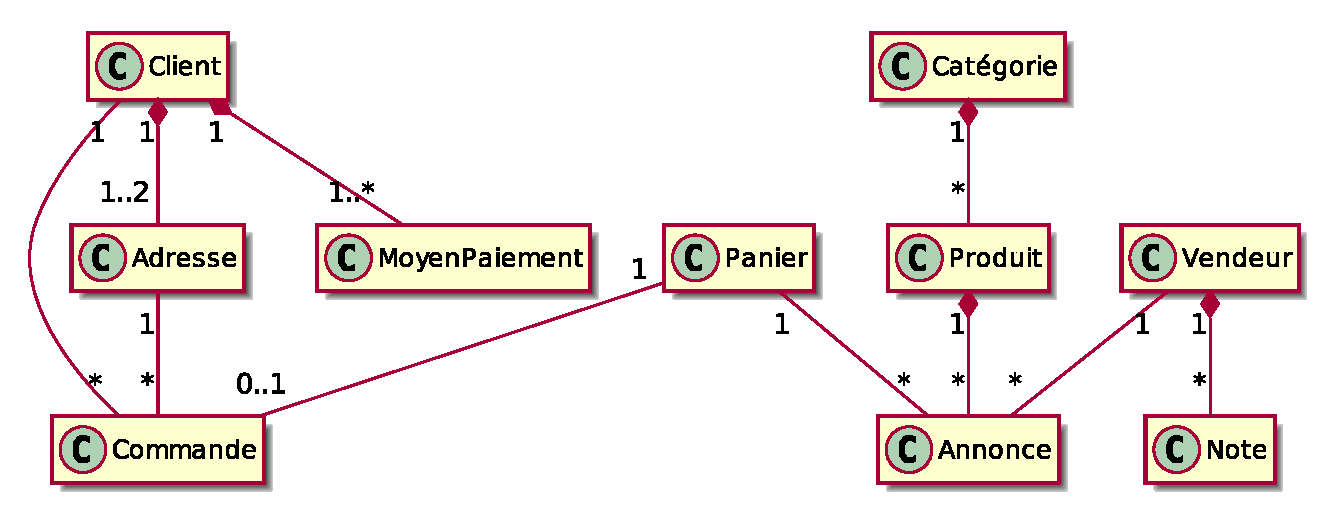
\includegraphics[width=15cm]{Images/MD} 

	\subsection{Diagramme de navigation}
	
	\includegraphics[trim = 6cm 1.5cm 5cm 2.2cm, clip]{Images/DN}
	
	\subsection{Identification des acteurs}
	
	Les acteurs humains pour le site Web sont :
	\begin{itemize}
		\item l'administrateur : en charge du bon fonctionnement (validation des annonces et des messages échangés) et de la maintenance du site   
		\item l'utilisateur non connecté : visiteur du site, n'a pas de compte 
		\item l'utilisateur connecté : possède un compte, peut acheter et vendre des objets
	\end{itemize}
	
	\subsection{Diagrammes de Cas d'Utilisation}
	\begin{itemize}
		\item DCU de l'Administrateur \\ 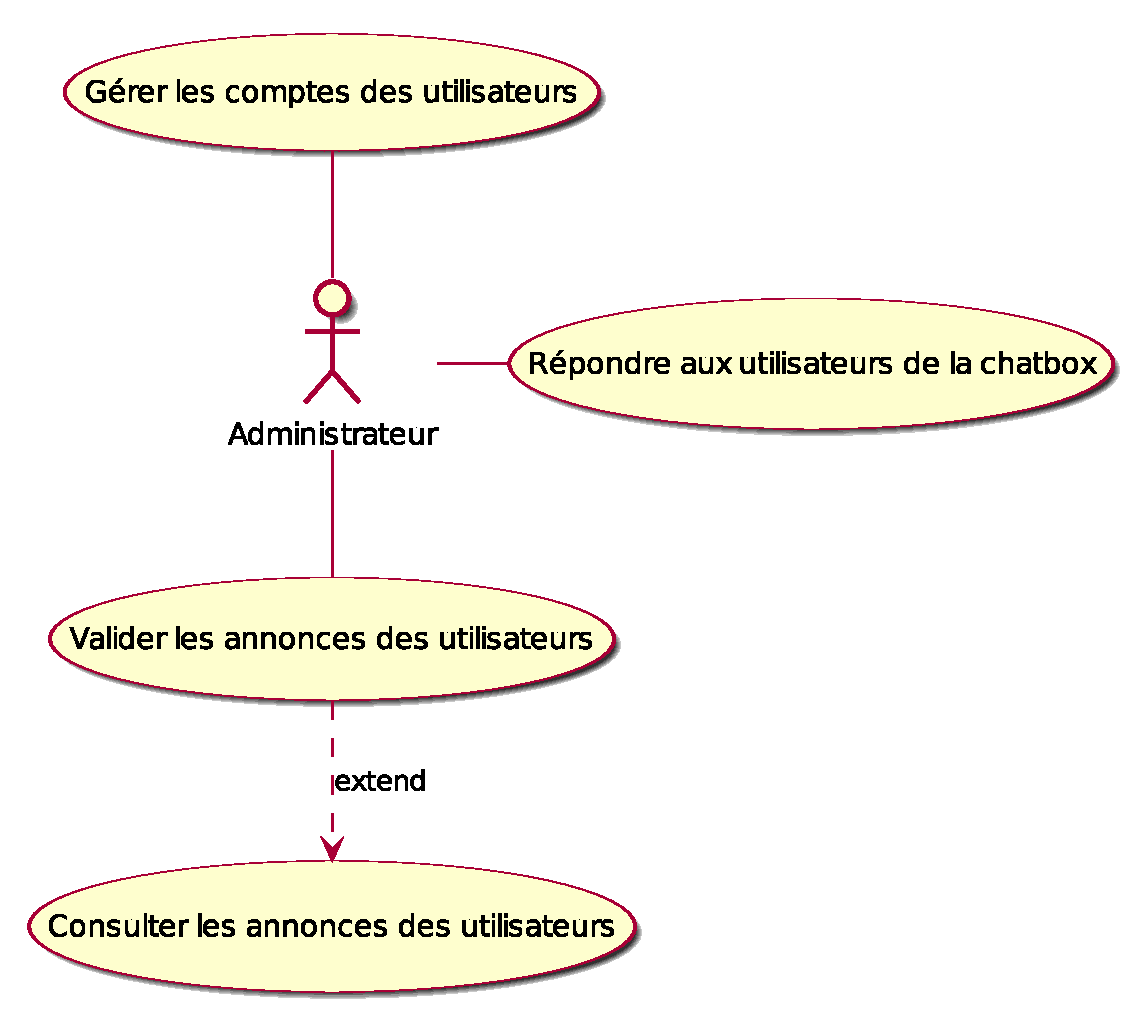
\includegraphics[height=10cm,width=15cm]{Images/DCU_Administrateur}
		\newpage
		\item DCU de l'Utilisateur Non Connecté \\
		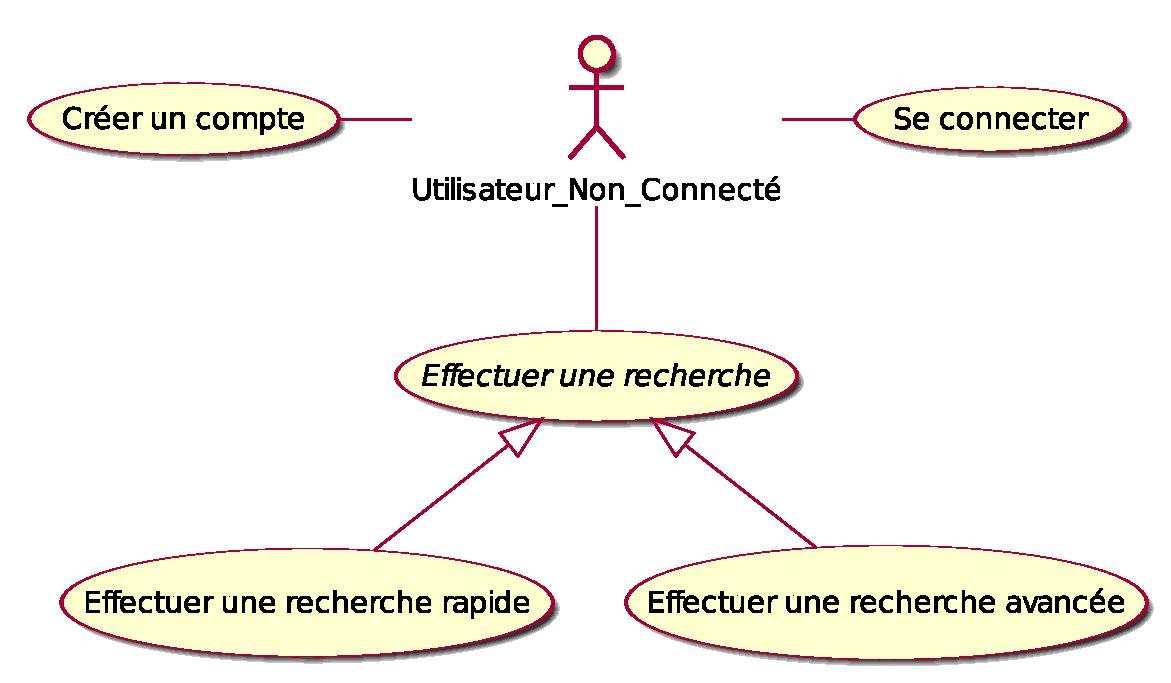
\includegraphics[height=7cm,width=15cm]{Images/DCU_UtilisateurNonConnecte} 
		\item DCU de l'Utilisateur Connecté \\
		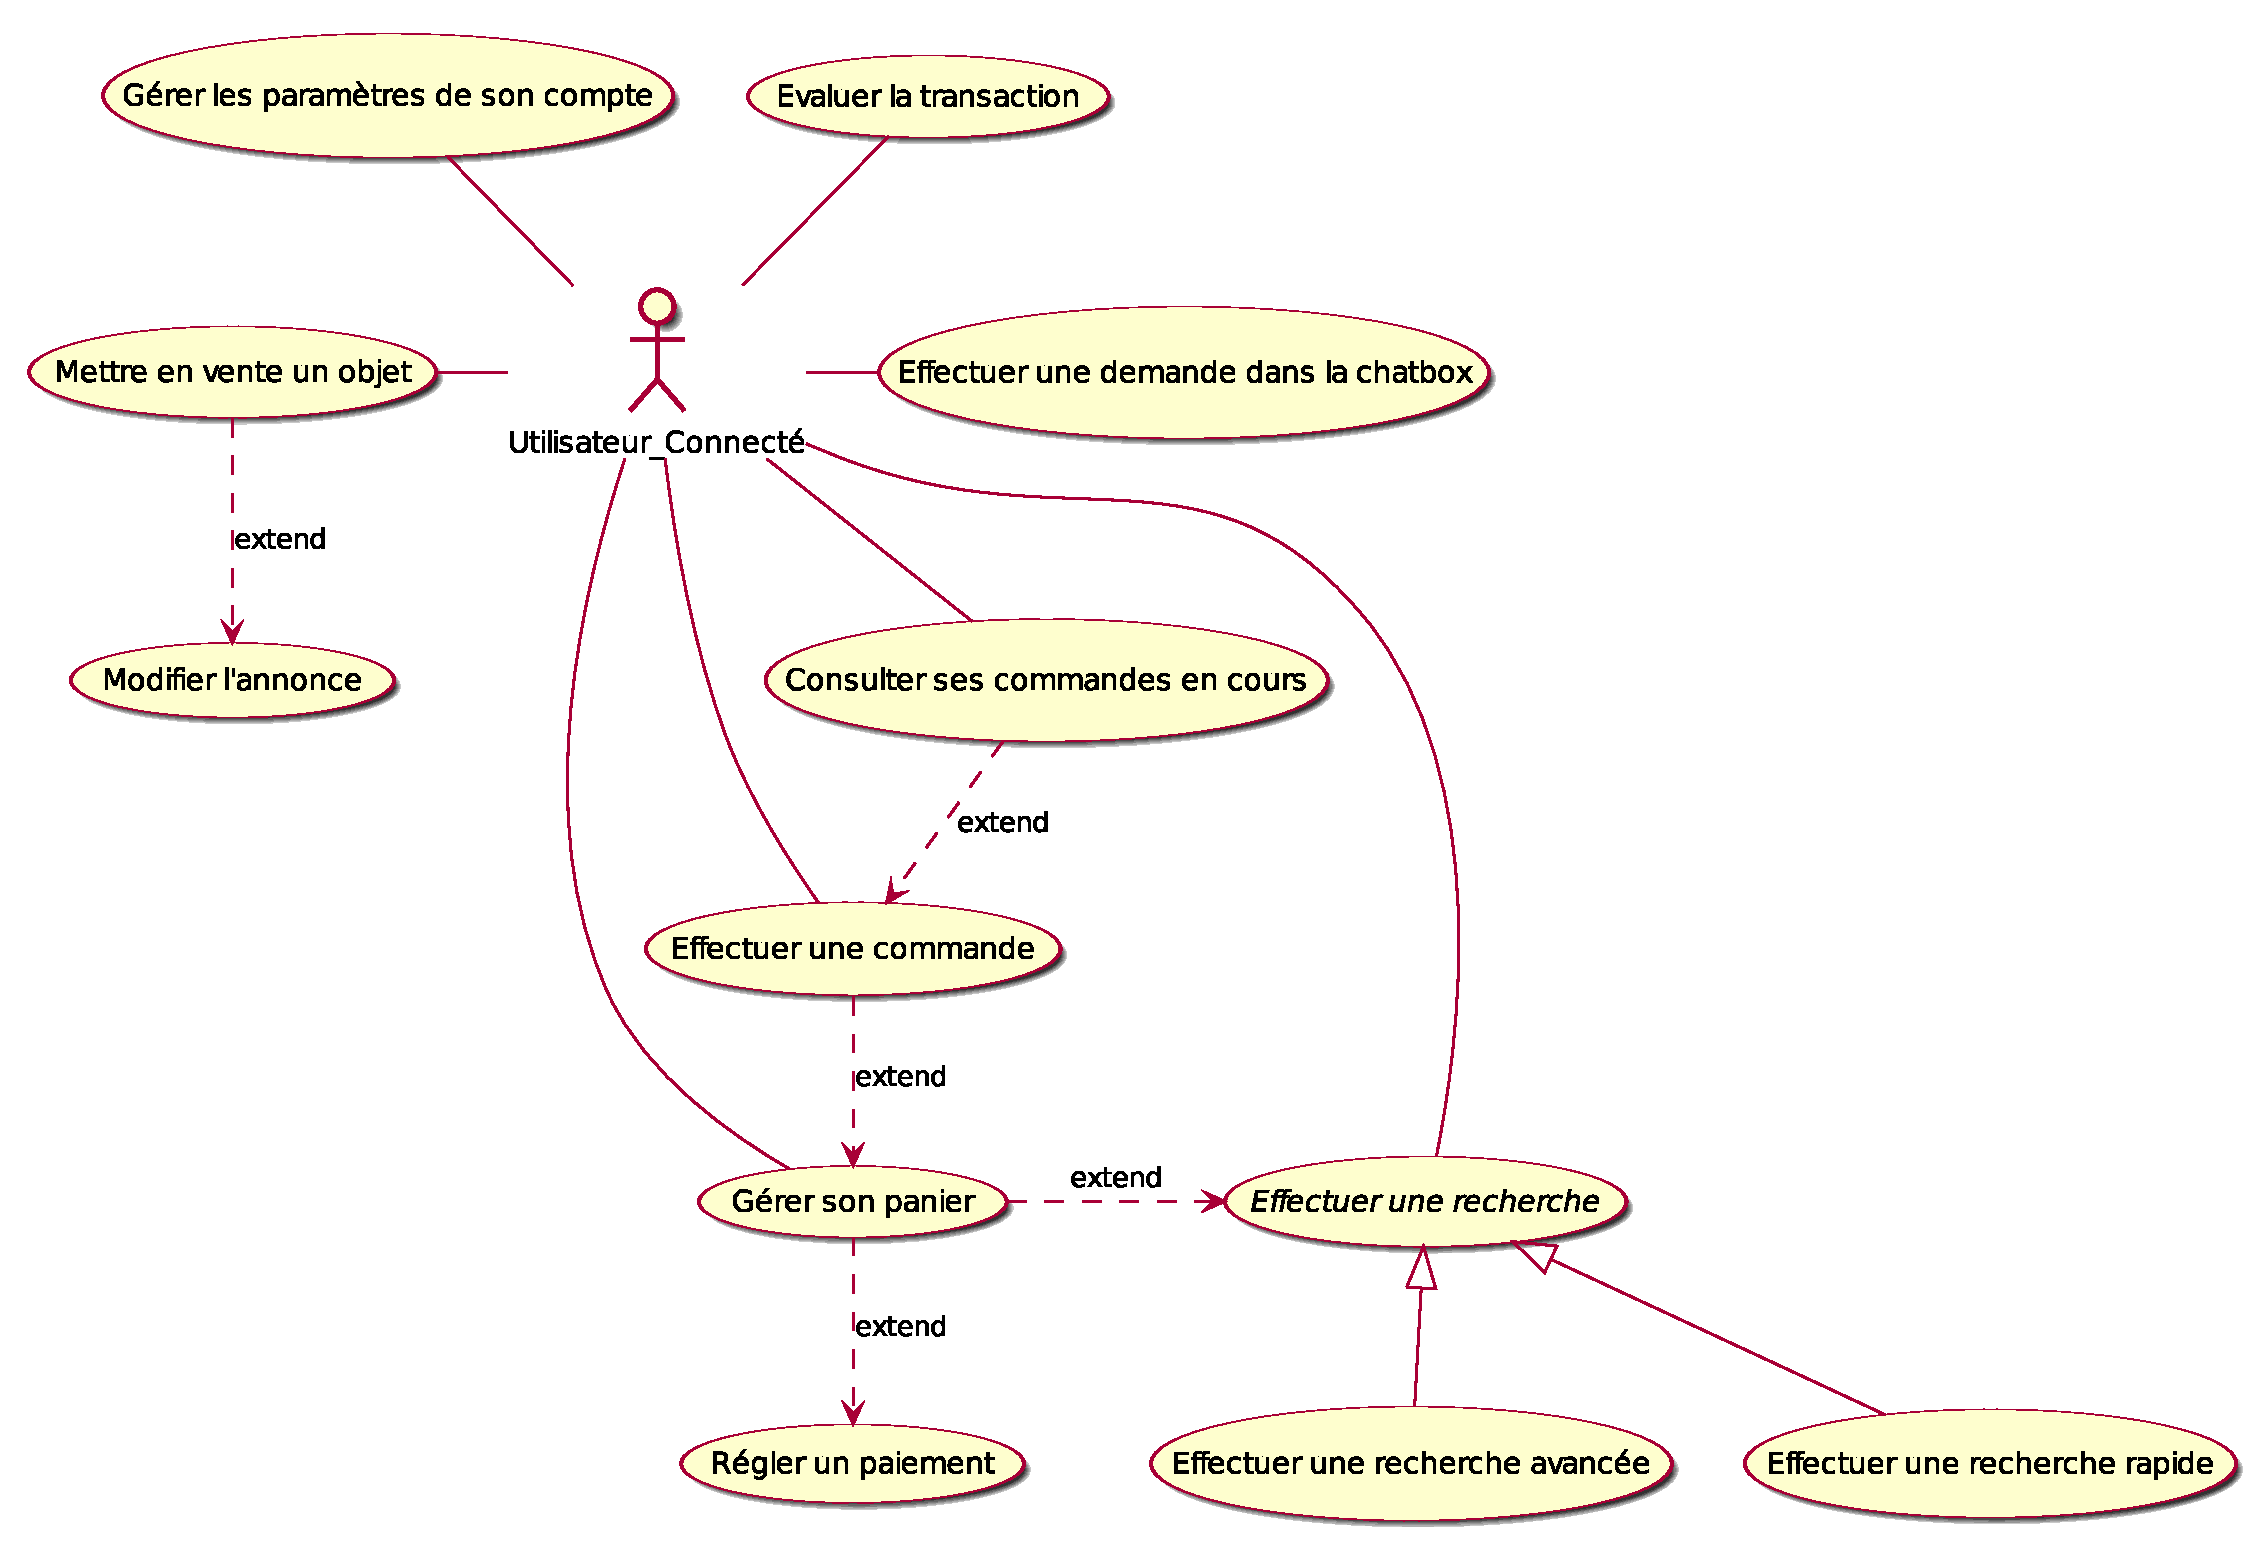
\includegraphics[width=17cm]{Images/DCU_UtilisateurConnecte} 
	\end{itemize}

\newpage
\section{Conception Préliminaire}
\subsection{Diagramme de classes de conception préliminaire}
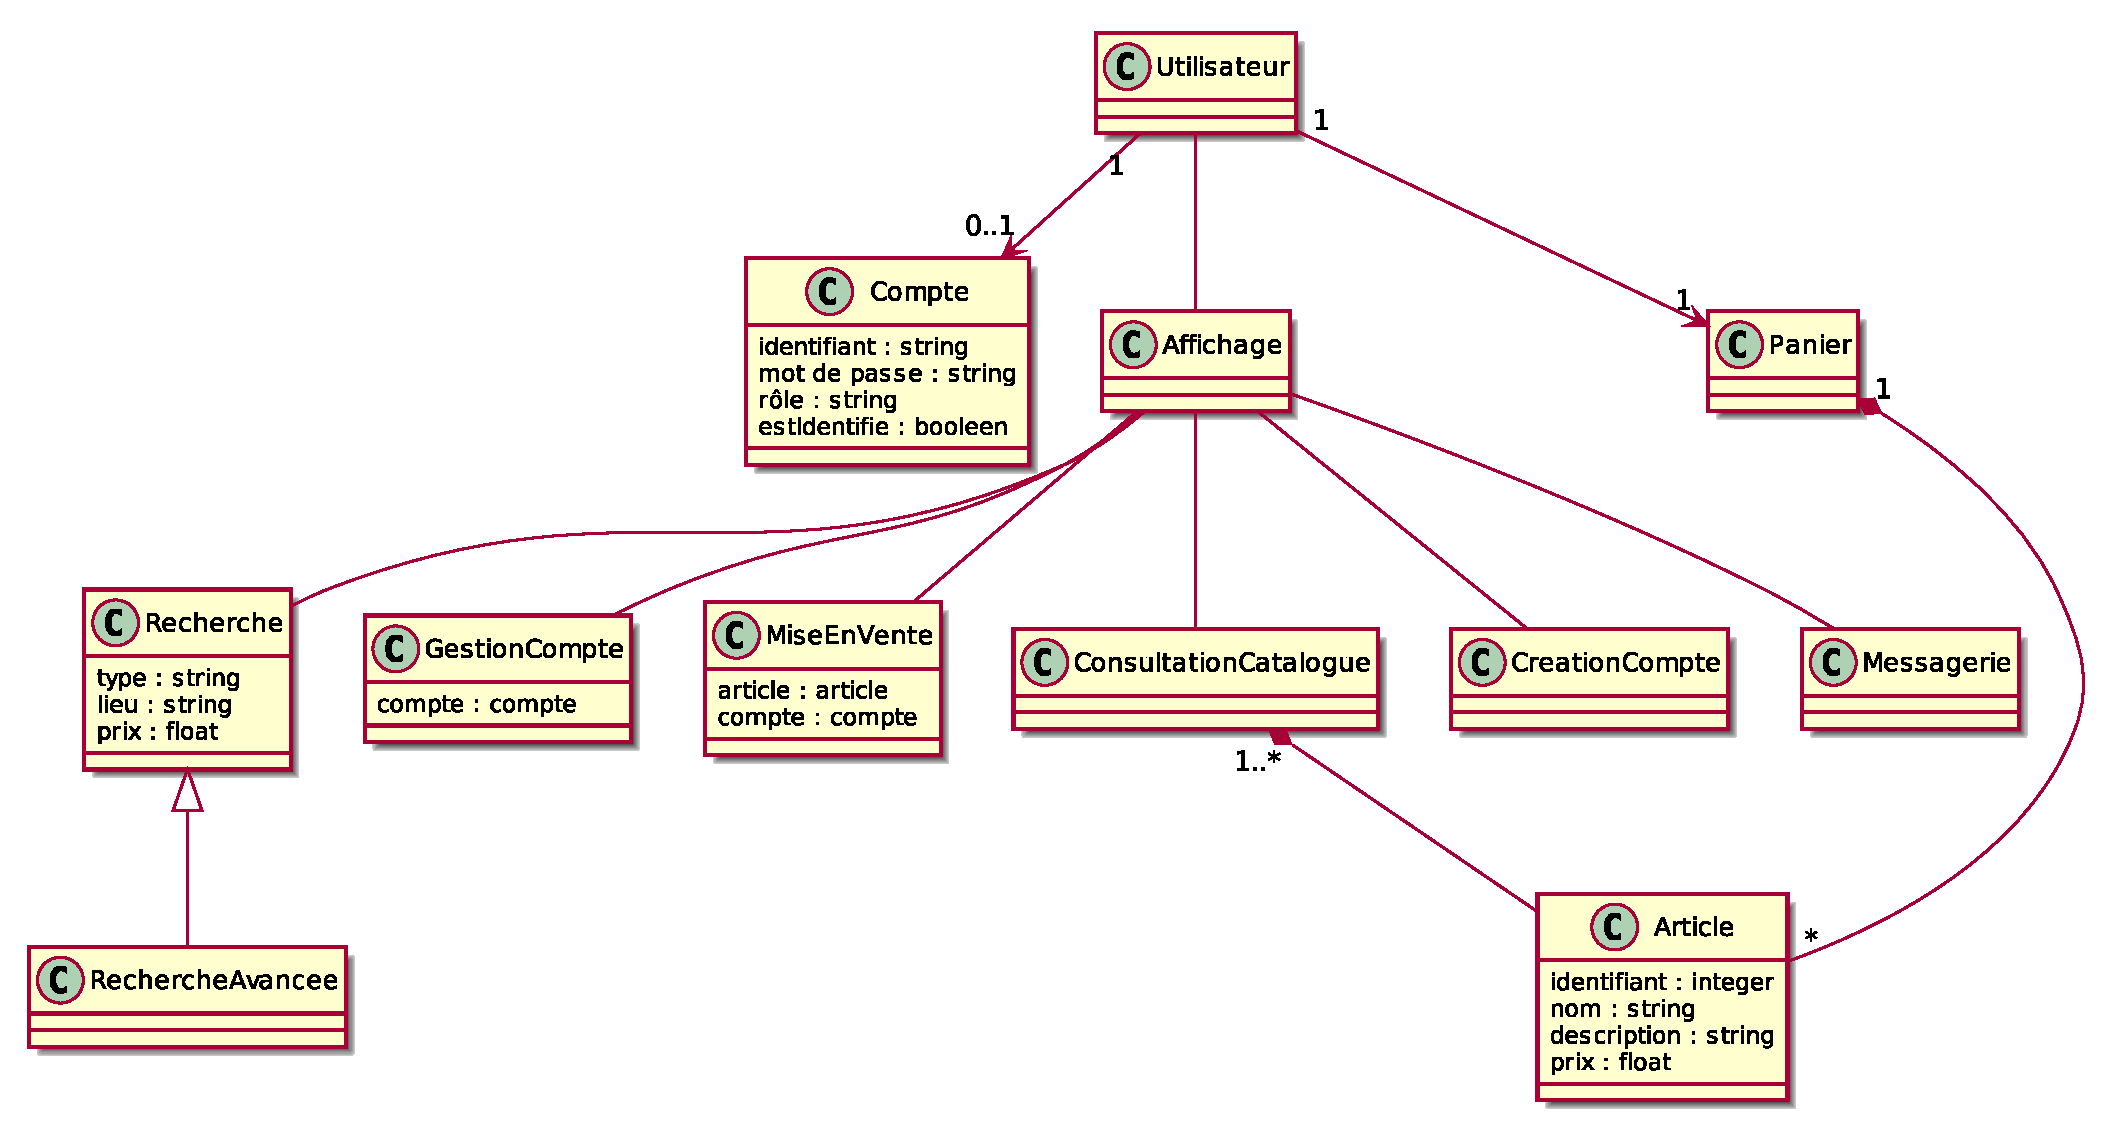
\includegraphics[width=17cm]{Images/DCCP} \\

\newpage
\subsection{Diagrammes de séquence}

\subsubsection{Création d'un compte}
Un visiteur peut créer un compte sur le site en renseignant ses informations et un mot de passe associé.\\
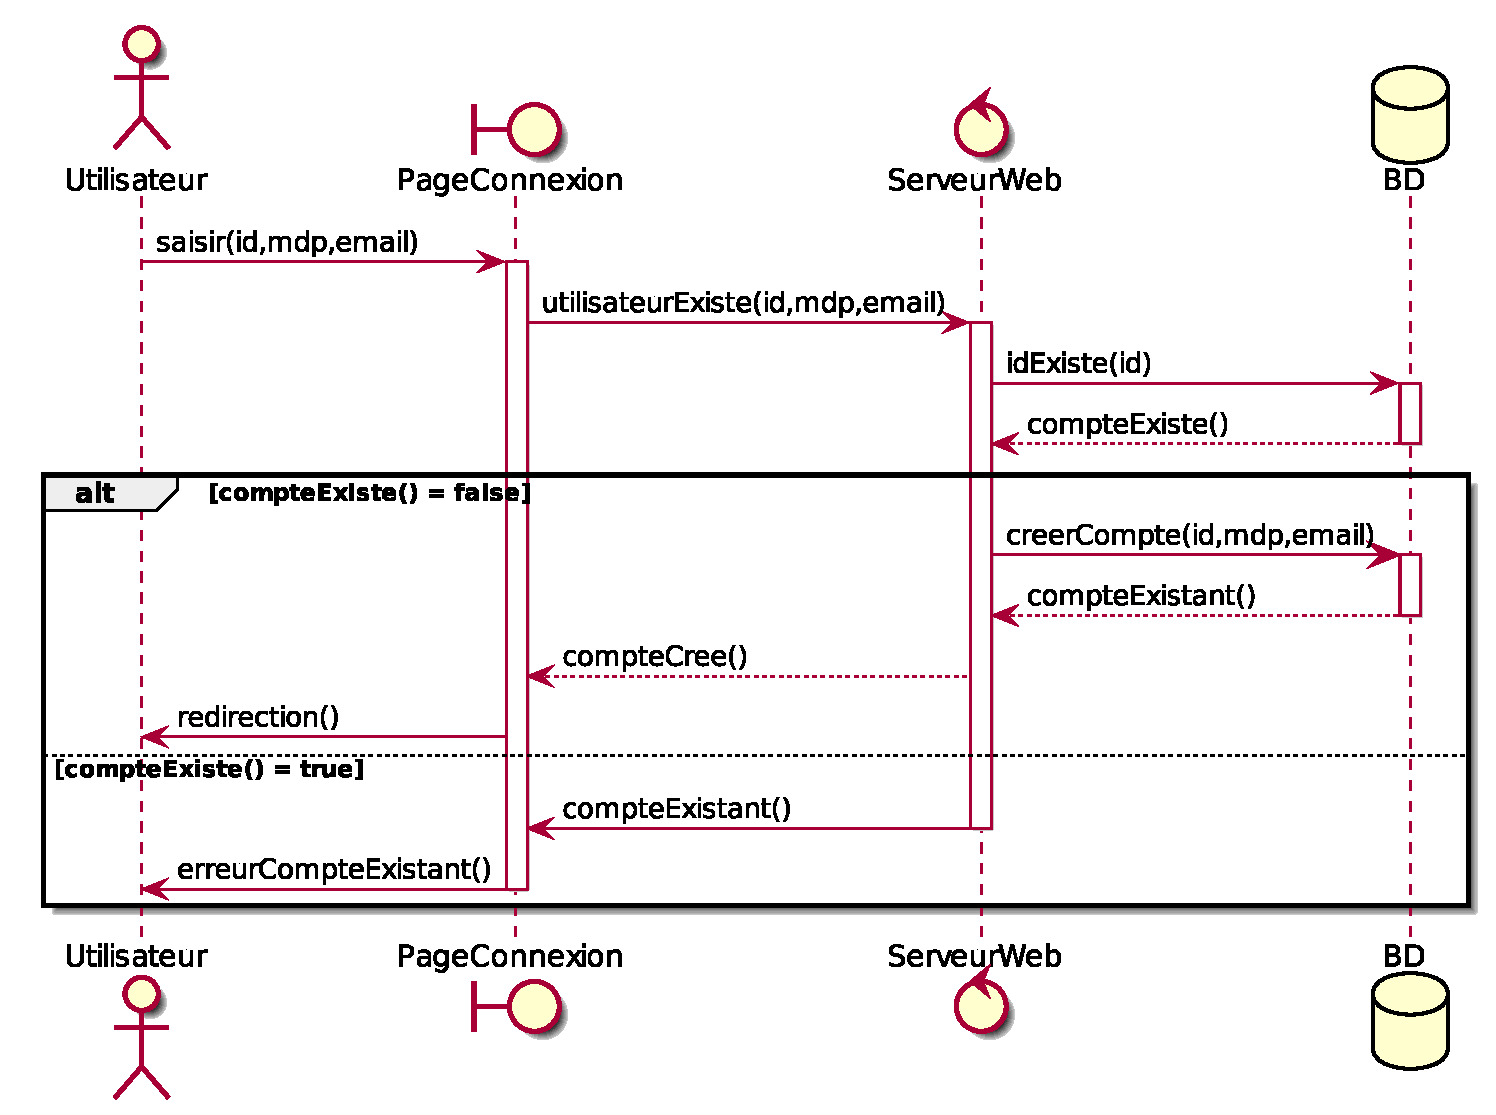
\includegraphics[width=15cm]{Images/DSEQ_CreationCompte} \\
\newpage
\subsubsection{Gestion d'un compte}
L'internaute peut procéder à la mise à jour de ses informations personnelles depuis la page de gestion du compte.\\
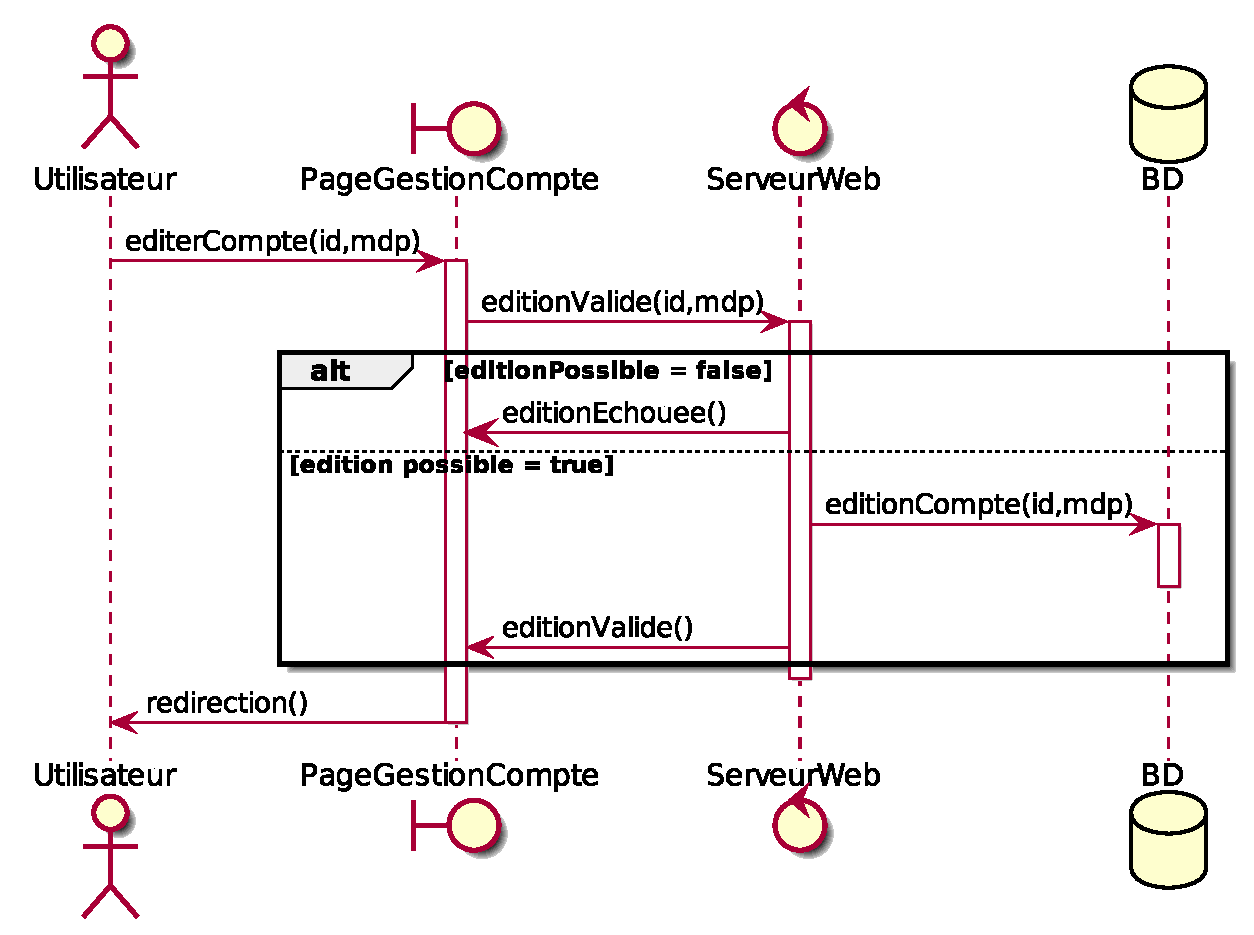
\includegraphics[width=17cm]{Images/DSEQ_GestionCompte} \\
\newpage
\subsubsection{Type de connexion}
Plusieurs type de connexion sont possibles : administrateur ou simple utilisateur \\
\includegraphics[width=17cm]{Images/DSEQ_TypeConnexion} \\
\newpage
\subsubsection{Recherche rapide ou avancée d'un objet}
Une fois sur le site, l'internaute souhaite trouver un objet à acheter selon ses critères. Pour cela, deux modes de recherche sont disponible, la recherche rapide selon une phrase entrée ou alors une recherche avancée selon le type, le prix et le lieu de vente de l'objet. \\
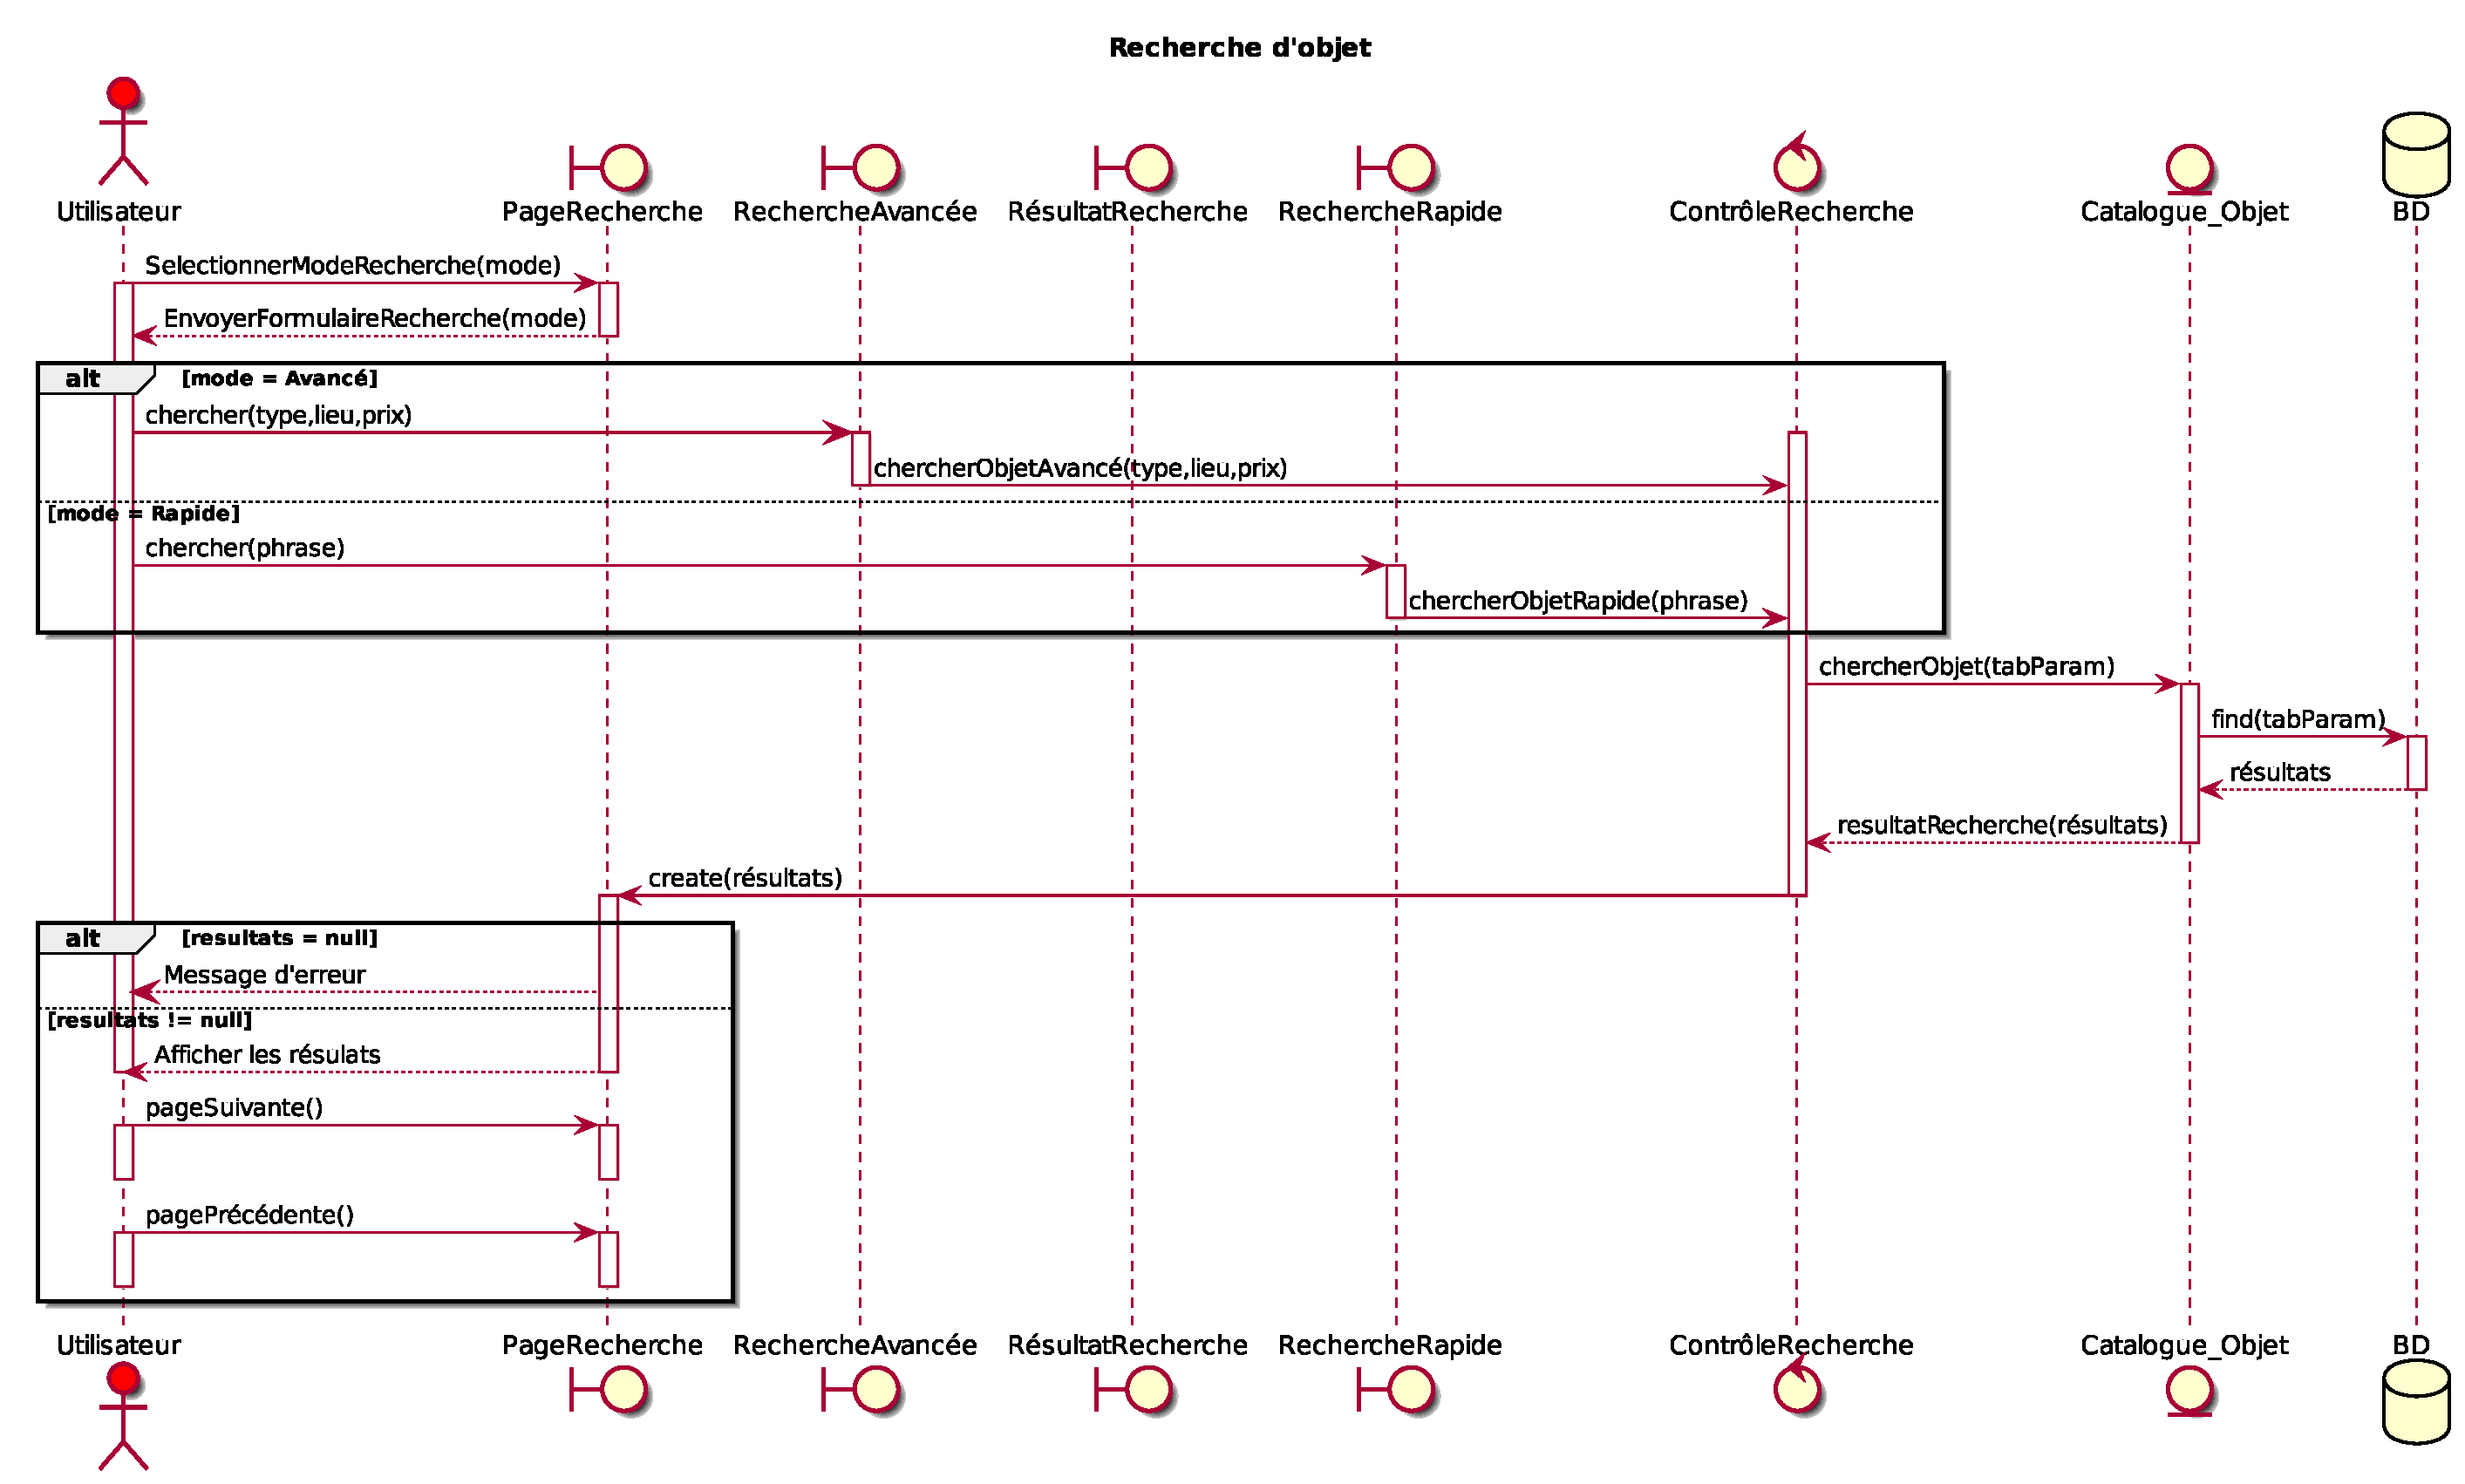
\includegraphics[width=17cm]{Images/DSEQ_Recherche} \\
\newpage
\subsubsection{Consultation d'un objet}
Lorsqu'une annonce intéressante est trouvée par l'internaute, il peut la consulter afin d'avoir des détails sur l'objet en vente tel que sa photo (facultative), son prix et sa description. \\
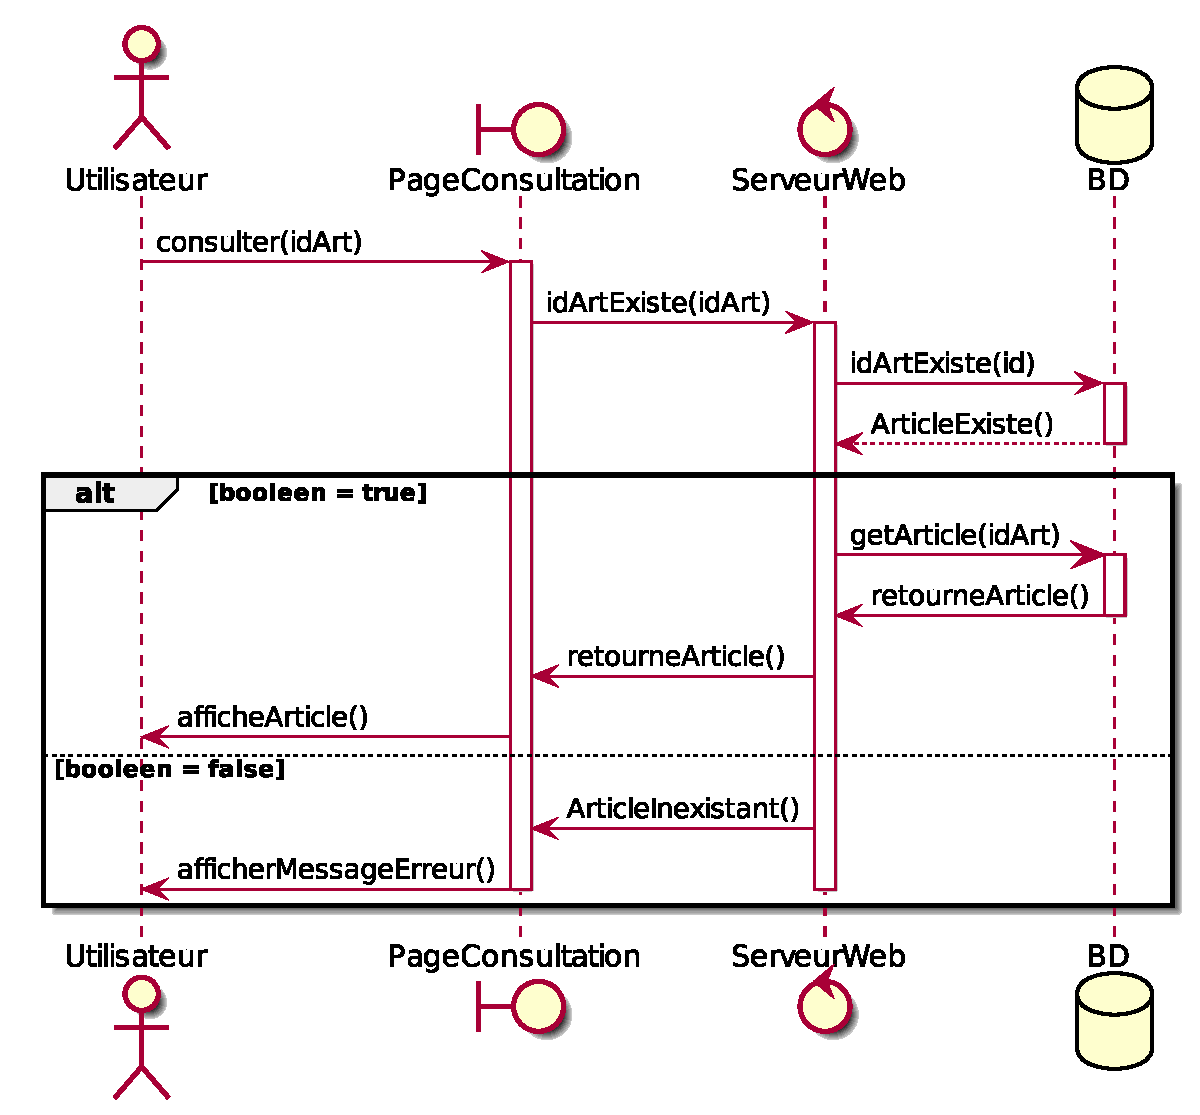
\includegraphics[width=17cm]{Images/DSEQ_Consultation} \\
\newpage
\subsubsection{Mise en vente}
L'internaute peut également mettre en vente un objet. Il doit renseigner les informations relatifs à l'objet pour que l'annonce puisse paraître. \\
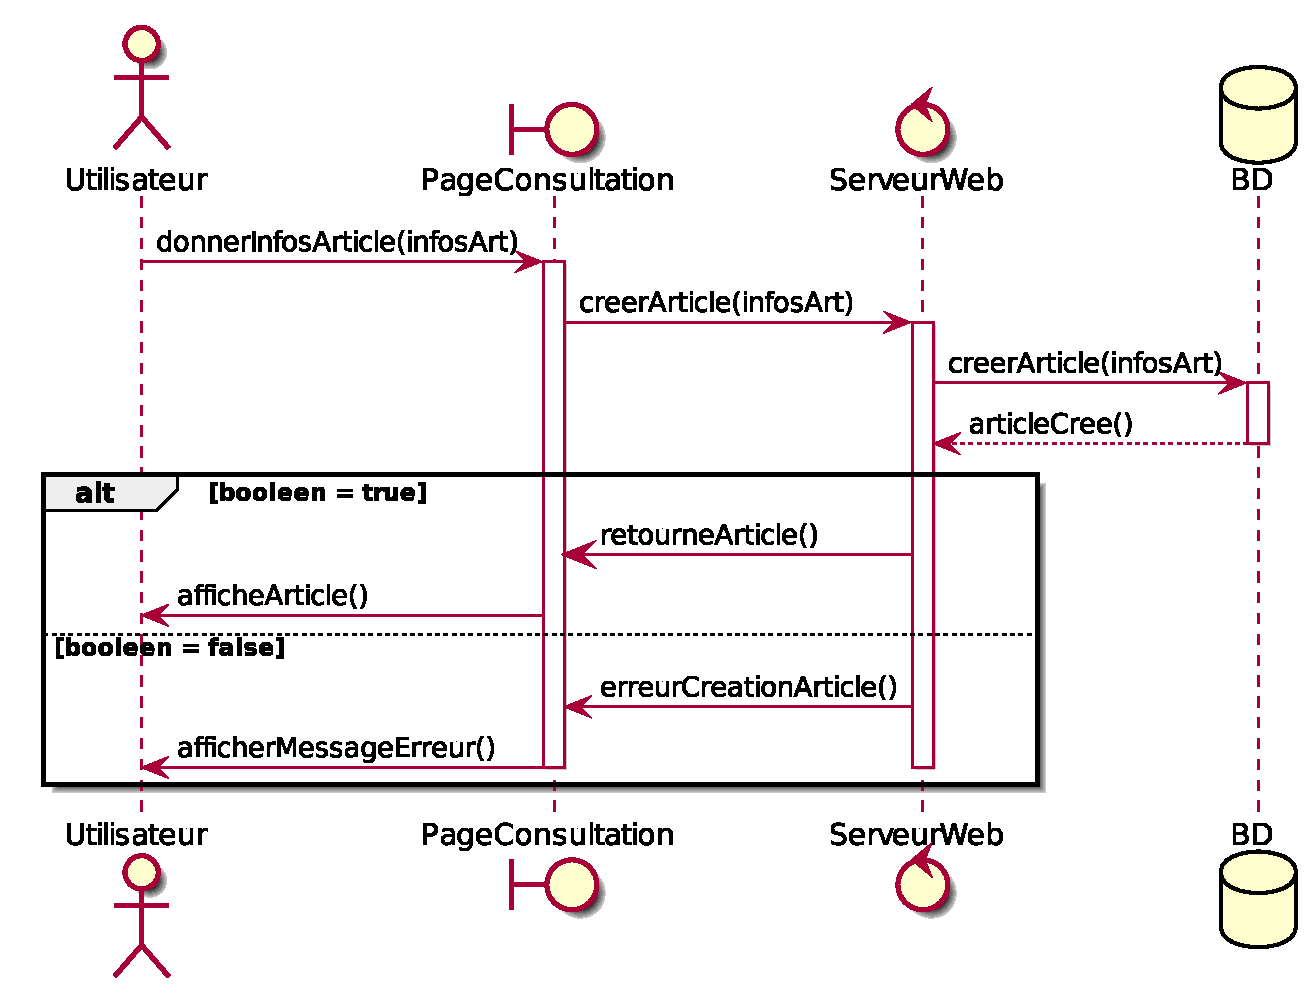
\includegraphics[width=17cm]{Images/DSEQ_MiseEnVente} \\
\newpage
\subsubsection{Panier}
L'internaute peut ajouter ou supprimer des articles de son panier en vue d'une commande. \\
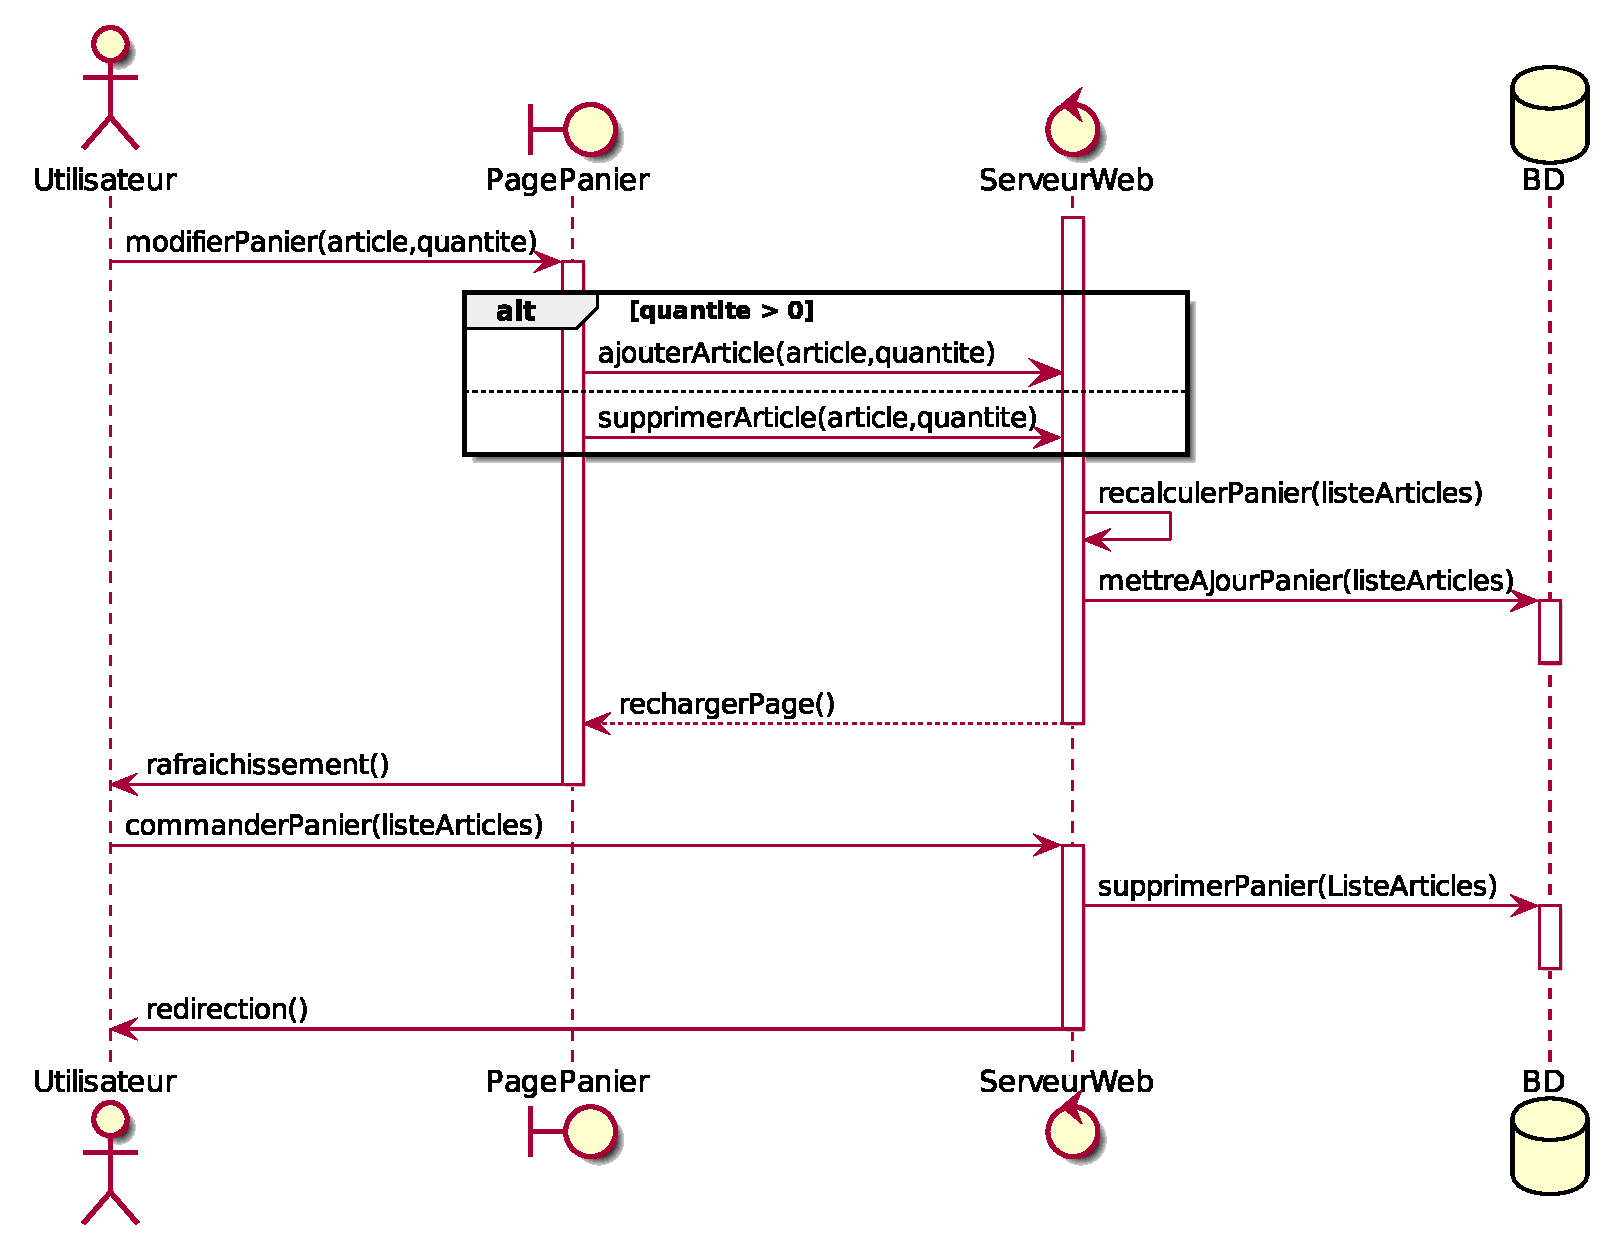
\includegraphics[width=17cm]{Images/DSEQ_Panier} \\
\newpage
\subsubsection{Paiement}
Lors de la mise en panier d'un ou plusieurs objets, l'internaute peut procéder au paiement en entrant ses coordonnées bancaires. \\
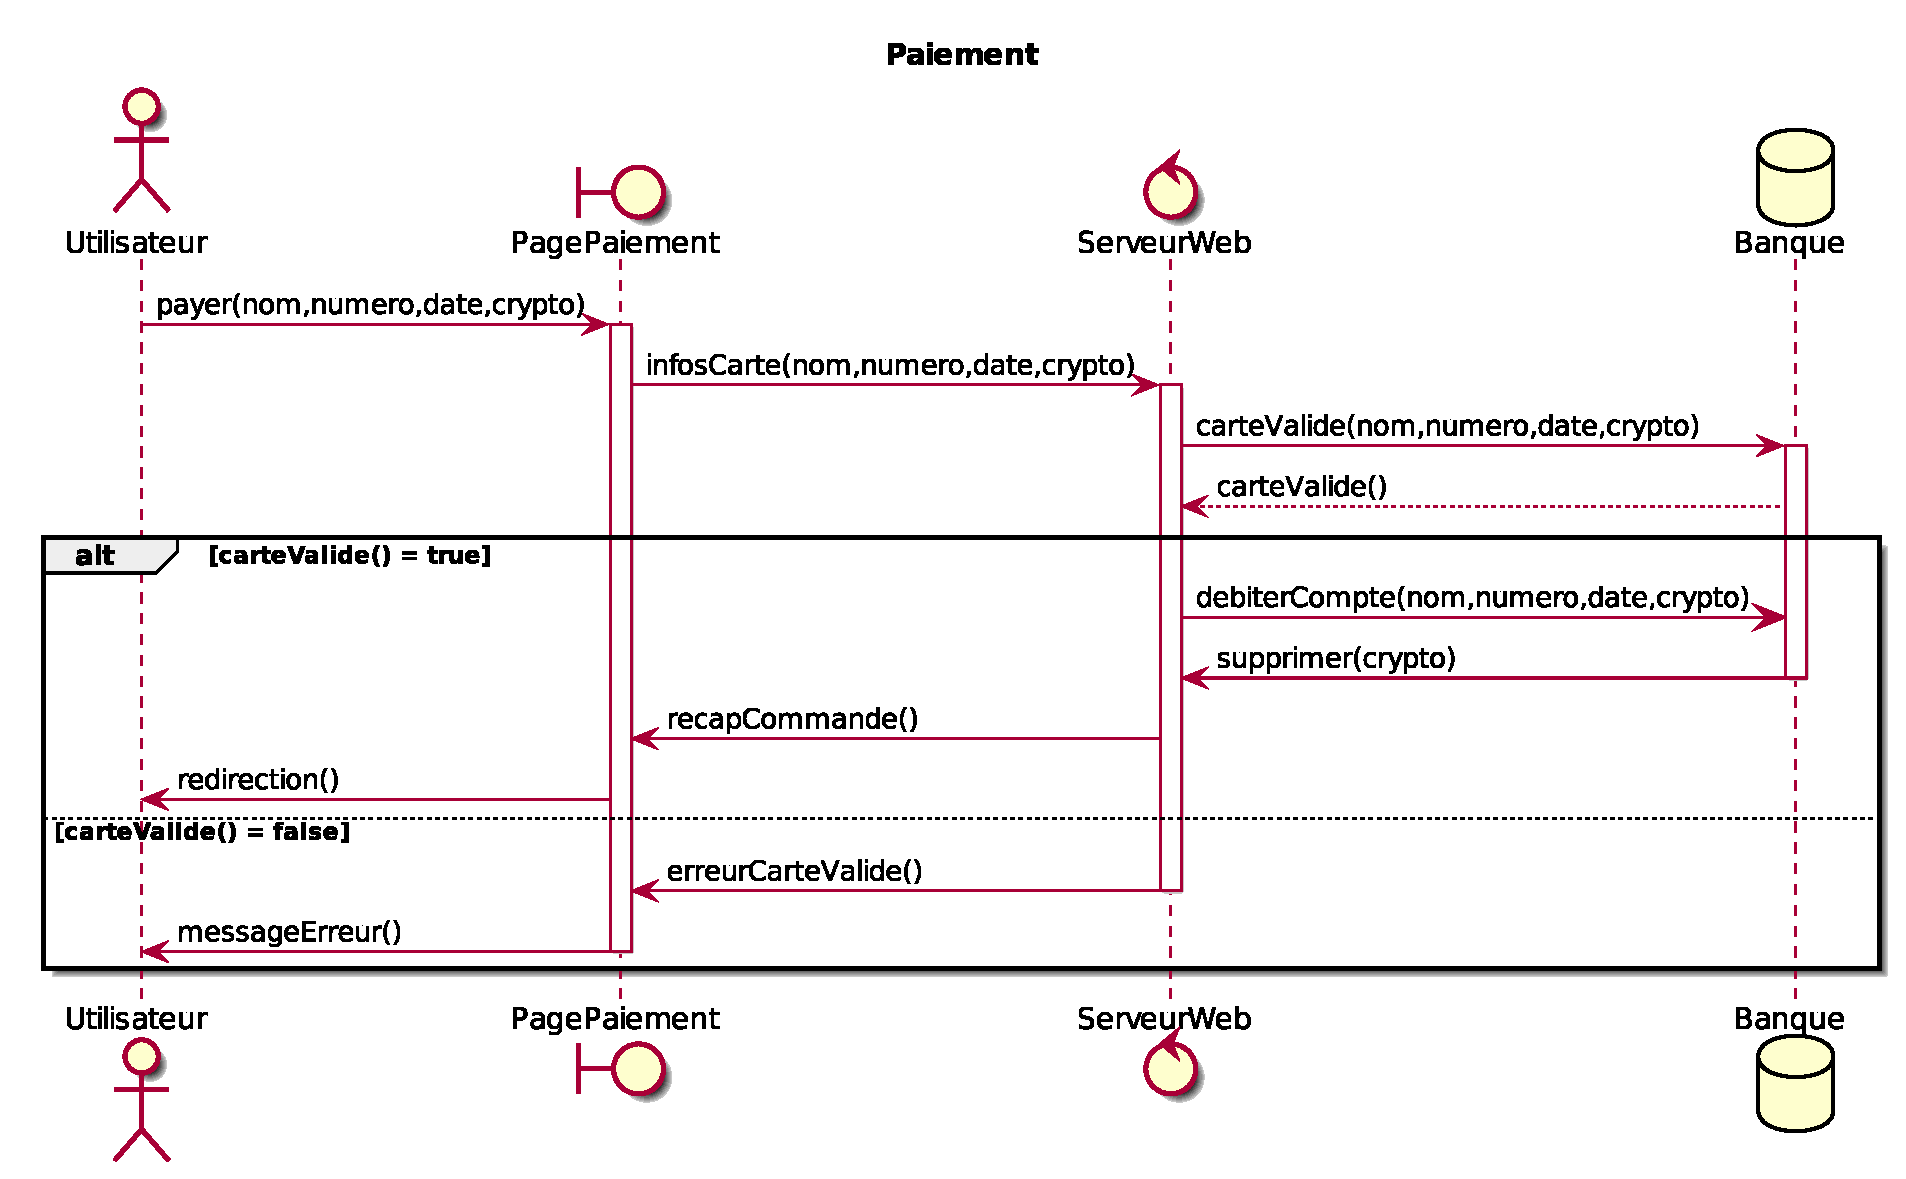
\includegraphics[width=17cm]{Images/DSEQ_Paiement} \\
\newpage
\subsubsection{Vote}
Lorsque la transaction est finalisée, l'internaute peut noter le vendeur. La note de celui-ci sera ainsi mise à jour. \\
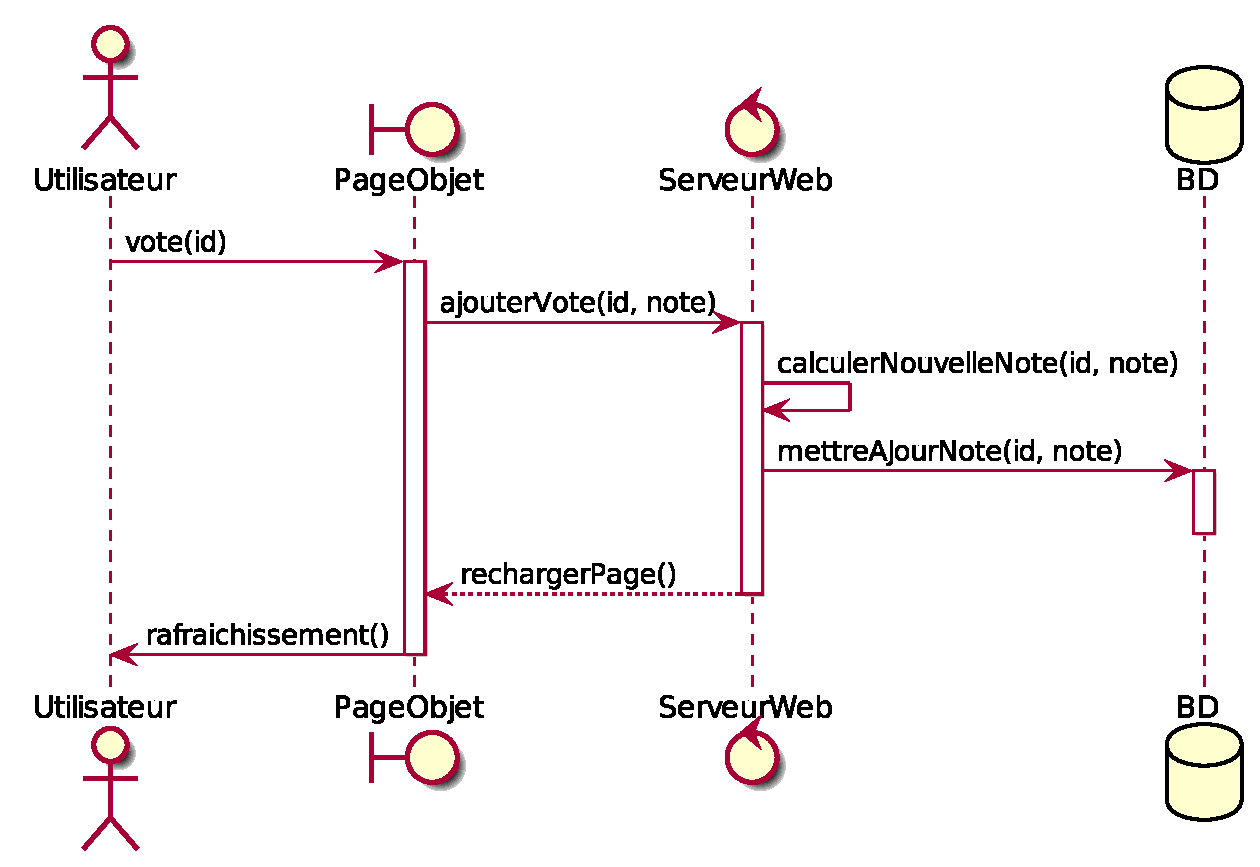
\includegraphics[width=17cm]{Images/DSEQ_Vote} \\
\newpage
\subsubsection{Messagerie}
Il est possible à l'internaute de demander des renseignements sur un objet mis en vente en envoyant un message au vendeur. Le contenu du message doit être validé au préalable par le modérateur. \\
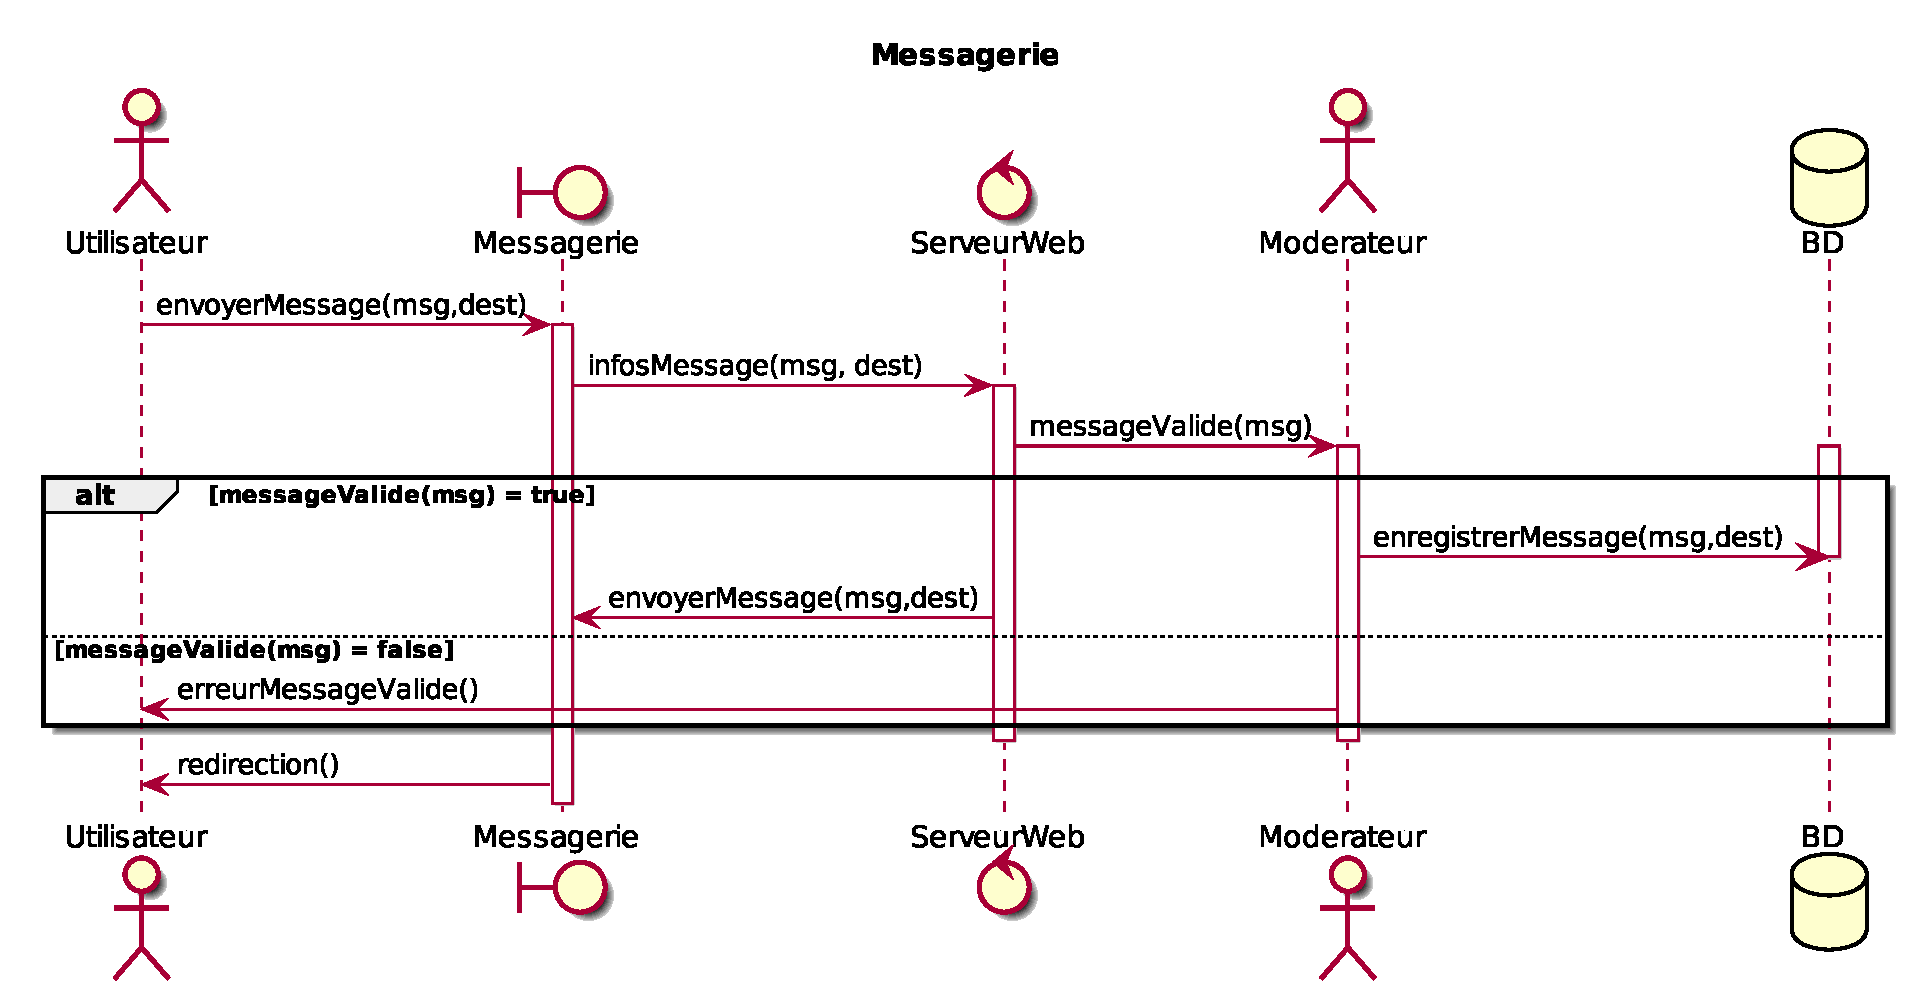
\includegraphics[width=17cm]{Images/DSEQ_Messagerie} \\


\newpage
\section{Conception Détaillée}
\subsection{Diagramme de classes}
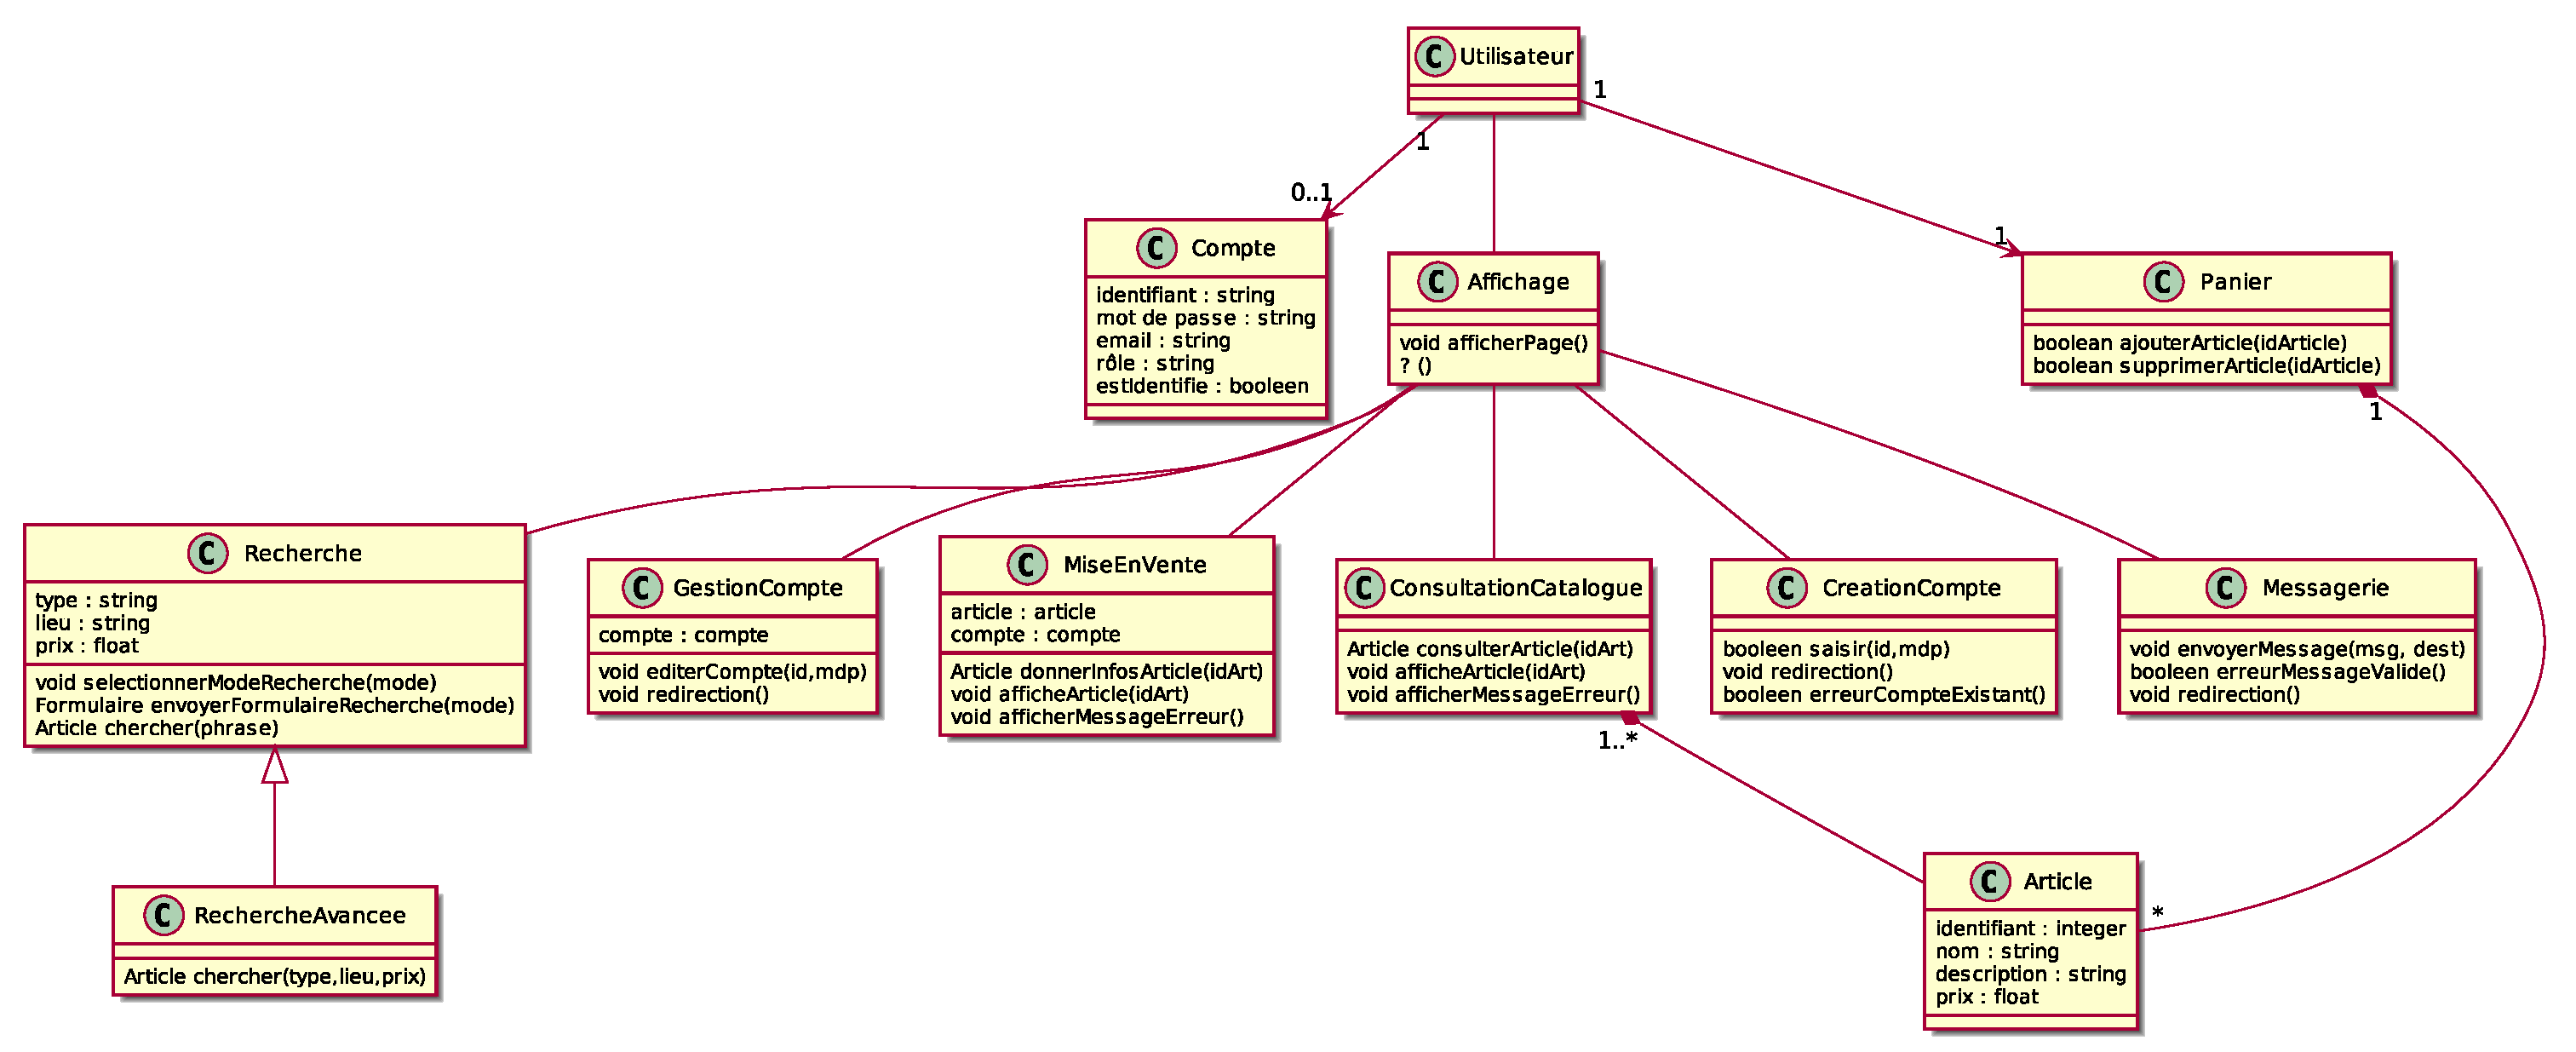
\includegraphics[width=15cm]{Images/DC}

\subsection{Diagramme de classes Struts}

\includegraphics[width=18cm]{Images/DC_Struts}

\subsection{Diagramme MVC}
\includegraphics[width=15cm]{Images/DiagrammeMVC.png}

\newpage
\section{Implémentation et tests}
\subsection{Implémentation}

Pour l'implémentation du site web, nous avons utilisé le framework Apache Struts. Il permet d'adopter plus facilement l'architecture Modèle-Vue-Contrôleur et comme nous l'avions déjà utilisé en cours, nous n'avons pas perdu de temps à apprendre les fonctionnalités.\\

Pour la gestion de la base de données, nous avons utilisé le système PostgreSQL. \\

Nous utilisons également l'architecture AJAX pour nos passages de paramètres sans formulaires, nous permettant d'effectuer des tâches asynchrones. Le format de données envoyées par les requêtes est le JSON. \\

Nous avons développé les points suivants :\\
\begin{itemize}
	\item Création d'un compte 
	\item Gestion d'un compte avec la modification du mot de passe
	\item Type de connexion 
	\item Gestion des sessions
	\item Recherche rapide ou avancée d'un objet
	\item Consultation d'un objet
	\item Consultation de profils utilisateurs
	\item Recherche et recherche avancée
	\item Mise en vente
	\item Gestion des annonces par administrateur
	\item Gestion des administrateurs
	\item Panier 
	\item Paiement via Paypal 
	\item Messagerie
\end{itemize}

Nous n'avions pas eu le temps de développer ces fonctionnalités : \\

\begin{itemize}
	\item Vote
	\item Gestion par l'utilisateur de ses articles déjà postés
\end{itemize}

\subsection{Tests}

Pour les tests, nous les avons fait manuellement sur le site web et enregistré ceux-ci dans une vidéo de démonstration :
\begin{itemize}
\item Tentative de connexion avec Pierre $\rightarrow$ pas de compte
\item Création du compte Pierre
\item Valider sans aucun champ $\rightarrow$ erreur 
\item Nouvelle tentative de création du compte Pierre $\rightarrow$ utilisateur déjà pris
\item Connexion avec le compte Pierre $\rightarrow$ mauvais mot de passe 
\item Connexion avec le bon mot de passe
\item Page votre compte
\item Recherche d’annonces (prix, description, catégorie, lieu)
\item Connexion avec le compte Flavien (déjà existant et admin)
\item Passer Pierre en admin
\item Déposer annonce
\item valider sans aucun champ $\rightarrow$ erreur
\item rechercher l'annonce déposée
\item Connexion du compte de Pierre (maintenant admin)
\item Valider l'annonce de Flavien
\item Rechercher l'annonce de Flavien 
\item Contacter Flavien (2messages)
\item Changer mot de passe de Pierre
\item Connexion compte Flavien $\rightarrow$ réponse
\item Connexion compte Pierre avec le nouveau mot de passe $\rightarrow$ réponse
\item Ajouter article Flavien  + un autre déjà présent
\item Paiement
\item Recherche des articles achetés $\rightarrow$ plus disponibles
\item Déconnexion
\end{itemize}


\newpage
\section{Conclusion et perspectives}
Nous n'avions pas eu le temps de développer ces fonctionnalités : 

\begin{itemize}
	\item Vote
	\item Gestion par l'utilisateur de ses articles déjà postés
\end{itemize}

Pour le vote, nous avons déjà mis en place les attributs nécessaires ainsi que les getters et setters associés dans Compte.java. Il faut maintenant lier le vendeur et l'acheteur afin qu'un acheteur puisse noter uniquement le vendeur associé à l'article qu'il a acheté. Sachant que nous pouvons déjà consulté l'identité d'un vendeur grâce à ses articles, il nous suffirait de rajouter un formulaire permettant à celui qui achète de noter celui ci.\\
Pour la gestion par l'utilisateur de ses articles déjà postés, cela ressemble beaucoup à la fonction "gestion des annonces par un administrateur" que nous avons déjà developpés. Il suffirait de reprendre cette fonctionnalité et de l'adapter à l'utilisateur afin qu'il puisse voir uniquement ses propres annonces.\\
Afin de vous faire une idée plus précise de notre site Web (en plus de la vidéo) nous avons également rendu celui-ci disponible sur internet afin de le tester directement. Il est disponible à l'addresse suivante : http://178.32.107.89:8080/Kristazax/index.jsp (Attention, le proxy de l'insa bloque l'accès au site). Nous vous fournissons également un accès administrateur afin d'acceder à toutes les fonctionnalités : utilisateur = testAdmin mdp = testAdmin123\\

\\



\newpage
\section{Bibliographie}
\begin{itemize}
	
\item Struts 2 File Upload Example \\
\url{http://www.mkyong.com/struts2/struts-2-file-upload-example/}

\item “UML : Modéliser un site e-commerce”, Pascal Roques, Eyrolles


\end{itemize}

\newpage
\section{Annexes}
\subsection{Maquette}

\subsubsection{Page d'accueil}
\includegraphics[width=13cm]{Images/maquette/Accueil} \\
\subsubsection{Page de création d'un compte}
\includegraphics[width=13cm]{Images/maquette/CreationCompte} \\
\subsubsection{Page de connexion}
\includegraphics[width=13cm]{Images/maquette/Login} \\
\subsubsection{Page de gestion du compte}
\includegraphics[width=13cm]{Images/maquette/VotreCompte} \\
\subsubsection{Page de présentation d'un objet}
\includegraphics[width=13cm]{Images/maquette/PageProduit}\\
\subsubsection{Page de recherche}
\includegraphics[width=13cm]{Images/maquette/ResultatRecherche}\\
\subsubsection{Page du panier}
\includegraphics[width=13cm]{Images/maquette/Panier}
\\
\subsubsection{Page de mise en vente}
\includegraphics[width=13cm]{Images/maquette/Vendre}

\end{document}

